% This is what we did
% Overview
%	numbers
%	gradient/non gradient participants
% Winners
%	Best Gradients

    There were 10 submissions for case study 1.
	One participant submitted twice, using a different optimization method for each submission.
	For anonymity, each submission was assigned a number.
	We refer to each submission below by this submission number (i.e., \textit{sub1}, ..., \textit{sub10}, etc.).
	For case study 2, there were 5 participant submissions.
	All five participants for case study 2 also submitted for case study 1, though were not required to do so.
	For ease of comparison, we assigned their submissions the same numbers from that case study as well
	(i.e., \textit{sub1} - \textit{sub5} are from the same individual participants for both case study 1 and case study 2).
	
	It should be noted that four of the authors submitted results for case study 1 as participants, and three submitted for case study 2.  The primary author developed and collecting data on the case study, but did so without sharing results with other participants including the other authors.  
	
% 	They did so independently, without collaboration, and without knowledge of the submitted results of any other participants.
% 	The development of the case study scenarios was also shared with all participants (not just the authors) prior to announcement.
	
	With submissions, was asked participants to also report their hardware specifications, and  performance data including function calls, wall time, and number of optimizations run.  Some of the questions in the exit questionnaire were not worded clearly enough, leading to different interpretations of time and function call reporting.  On case showing wall time is shown below.
% 	Some submitted data for individual optimizations, others for all their optimizations together.
% 	Because this data for the most part uncomparable, the only metric included in this report is for the 64 turbine case of case study 2 in \cref{fig:AEPvTime}, that measures AEP vs reported wall time for all runs.

\subsection{Case Study 1: Optimization Only}\label{sec:res-optonly}

	Participants ran the optimization algorithm of their choosing using our supplied AEP function or a functional equivalent in another language.
	%Since there exists a great deal of variability in hardware, participants also reported processor speed, function calls, number of cores used, and total Random Access Memory (RAM) installed in their system when finding their optimized results.
	The AEP results and rankings are given below in \cref{tab:results1,tab:results2,tab:results3}.

	\subsubsection{Data}

	\cref{tab:results1,tab:results2,tab:results3} display the final AEP data of all participant-proposed optimal turbine layouts.
	The Python module we supplied, which uses the simplified Bastankhah wake model, was used for all AEP calculations.
	Submissions were ranked from highest to lowest resultant AEP values.
	Also listed in the tables are the submission number (sub\#), whether a gradient-based (G) or gradient-free (GF) optimization method was used, and the relative percentage increase of AEP (Increase) from the provided example layout's AEP.
	
% 	\newpage
		\begin{table}[htbp]
			\begin{center}
				\caption{16 turbine scenario participant results}
				\label{tab:results1}
				\begin{tabular}{r l l c r r}
					\hline
					Rank	& Algorithm											& sub\#	& Grad.	& AEP			& Increase		\\	%& Norm.		\\
					\hline
					1       & SNOPT\texttt{+}WEC								& 4     & G		& 418924.4064	&	14.17 \% 	\\ %&	- \% 	\\
					2       & fmincon											& 5     & G		& 414141.2938	&	12.86 \% 	\\ %&	-1.14 \% 	\\
					3       & SNOPT												& 8     & G		& 412251.1945	&	12.35 \% 	\\ %&	-1.59 \% 	\\
					4       & SNOPT												& 1     & G		& 411182.2200	&	12.06 \% 	\\ %&	-1.85 \% 	\\
					5       & Preconditioned Sequential Quadratic Programming	& 2     & G		& 409689.4417	&	11.65 \% 	\\ %&	-2.20 \% 	\\
					6       & Multistart Interior-Point							& 10    & G		& 408360.7813	&	11.29 \% 	\\ %&	-2.52 \% 	\\
					7       & Full Pseudo-Gradient Approach						& 3     & GF	& 402318.7567	&	9.64 \% 	\\ %&	-3.96 \% 	\\
					8       & Basic Genetic Algorithm							& 7     & GF	& 392587.8580	&	6.99 \% 	\\ %&	-6.29 \% 	\\
					9       & Simple Particle Swarm Optimization				& 6     & GF	& 388758.3573	&	5.95 \% 	\\ %&	-7.20 \% 	\\
					10      & Simple Pseudo-Gradient Approach					& 9     & GF	& 388342.7004	&	5.83 \% 	\\ %&	-7.30 \% 	\\
					11		& (Example Layout)									& -		& -		& 366941.5712	&	- 			\\ %&	-12.41 \% 	\\
					\hline
				\end{tabular}
			\end{center}
% 		\end{table}

	%\subsubsection{36 Turbine Case}

% 		\begin{table}[htbp]
			\begin{center}
				\caption{36 turbine scenario participant results}
				\label{tab:results2}
				\begin{tabular}{r l c c l r}
					\hline
					Rank	& Algorithm											& sub\#	& Grad.	& AEP			& Increase		\\	%& Norm.		\\
					\hline
					1		& SNOPT\texttt{+}WEC								& 4		& G		& 863676.2993   &	17.05 \% 	\\ %&	- \% 	\\
					2		& Multistart Interior-Point							& 10	& G		& 851631.9310	&	15.42 \% 	\\ %&	-1.39 \% 	\\
					3		& Preconditioned Sequential Quadratic Programming	& 2     & G		& 849369.7863	&	15.11 \% 	\\ %&	-1.66 \% 	\\
					4		& SNOPT												& 8     & G		& 846357.8142	&	14.70 \% 	\\ %&	-2.01 \% 	\\
					5		& SNOPT												& 1     & G		& 844281.1609	&	14.42 \% 	\\ %&	-2.25 \% 	\\
					6		& Full Pseudo-Gradient Approach						& 3     & GF	& 828745.5992	&	12.31 \% 	\\ %&	-4.04 \% 	\\
					7		& fmincon											& 5     & G		& 820394.2402	&	11.18 \% 	\\ %&	-5.01 \% 	\\
					8		& Simple Pseudo-Gradient Approach					& 9     & GF	& 813544.2105	&	10.25 \% 	\\ %&	-5.80 \% 	\\
					9		& Basic Genetic Algorithm							& 7     & GF	& 777475.7827	&	5.37 \% 	\\ %&	-9.98 \% 	\\
					10		& Simple Particle Swarm Optimization				& 6     & GF	& 776000.1425	&	5.17 \% 	\\ %&	-14.56 \% 	\\
					11		& (Example Layout)									& -		& -		& 737883.0985	&	- 			\\ %&	-14.57 \% 	\\
					\hline
				\end{tabular}
			\end{center}
% 		\end{table}

	%\subsubsection{64 Turbine Case}

% 		\begin{table}[htbp]
			\begin{center}
				\caption{64 turbine scenario participant results}
				\label{tab:results3}
				\begin{tabular}{r l c c l r}
					\hline
					Rank	& Algorithm											& sub\#	& Grad.	& AEP			& Increase		\\	%& Norm.		\\
					\hline
					1		& SNOPT\texttt{+}WEC								& 4 	& G		& 1513311.1936	&	16.86 \% 	\\ %&	- \% 	\\
					2		& Preconditioned Sequential Quadratic Programming	& 2		& G		& 1506388.4151	&	16.36 \% 	\\ %&	-0.46 \% 	\\
					3		& Multistart Interior-Point							& 10	& G		& 1480850.9759	&	14.35 \% 	\\ %&	-2.15 \% 	\\
					4		& SNOPT												& 1		& G		& 1476689.6627 	&	14.03 \% 	\\ %&	-2.42 \% 	\\
					5		& Full Pseudo-Gradient Approach						& 3		& GF	& 1455075.6084	&	12.36 \% 	\\ %&	-3.85 \% 	\\
					6		& SNOPT												& 8		& G		& 1445967.3772	&	11.66 \% 	\\ %&	-4.45 \% 	\\
					7		& Simple Pseudo-Gradient Approach					& 9		& GF	& 1422268.7144	&	9.82 \% 	\\ %&	-6.02 \% 	\\
					8		& Simple Particle Swarm Optimization				& 6		& GF    & 1364943.0077	&	5.40 \% 	\\ %&	-9.80 \% 	\\
					9		& fmincon											& 5		& G		& 1336164.5498 	&	3.18 \% 	\\ %&	-11.71 \% 	\\
					10		& Basic Genetic Algorithm							& 7		& GF	& 1332883.4328	&	2.93 \% 	\\ %&	-11.92 \% 	\\
					11		& (Example Layout)									& -		& -		& 1294974.2977	&	- 			\\ %&	-14.43 \% 	\\
					\hline
				\end{tabular}
			\end{center}
		\end{table}

		%\begin{table}[htbp]
		%	\begin{center}
		%		\caption{16 turbine scenario participant results}
		%		\label{tab:results1}
		%		\begin{tabular}{r l l l l r}
		%			\hline
		%			sub\#		& Wake Model 			& Algorithm									\\	
		%			\hline
		%			1		& FLORISSE 3D			& SNOPT											\\
		%			2		& Park2					& PSQP											\\
		%			3		& Bastankhah			& Full Pseudo-Gradient Approach					\\
		%			4		& Bastankhah			& SNOPT\texttt{+}WEC 							\\
		%			5 		& Simplified Bastankhah	& fmincon										\\
		%			\hline
		%		\end{tabular}
		%	\end{center}
 		%\end{table}

% 		\begin{figure}[H]
% 			\centering 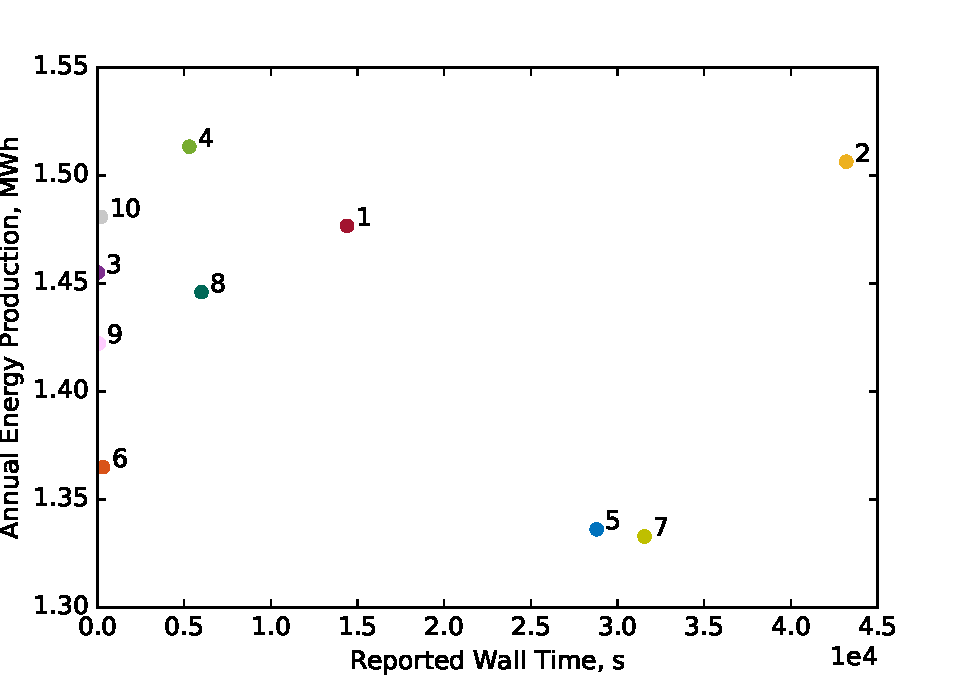
\includegraphics[width=.8\textwidth]{./figures/AEP_vs_time.pdf}
% 			\caption{AEP vs reported wall time for each submitted optimization method of the 64 turbine scenario}
% 			\label{fig:AEPvsTime}
% 		\end{figure}
	
	\import{./sections/}{iea37-wflocs-rslts-optonly.tex}

\subsection{Case Study 2: Combined Physics Model/Optimization Algorithm}\label{sec:res-cmbnd}

	For case study 2, participants ran both the optimization algorithm and wake model of their choosing.
	There was no restrictions on programming language for either the wake model or optimization algorithm, but results of optimal turbine layouts were to be submitted in the \texttt{.yaml} format supplied in the case study 1 examples.

	Because participants used different wake models, AEP values reported cannot be fairly compared between participants.
	Results were therefore judged on cross-comparison calculations.

	\subsubsection{Data}

	The cross-comparison displays some interesting trends.
	\cref{tab:sub1cc,tab:sub2cc,tab:sub3cc,tab:sub4cc,tab:sub5cc} show how each submission's wake models ranked the proposed optimal turbine layouts for the other 4 submissions.
	Each submission's ranking of its own layout is in \textbf{bold}.
	The penultimate column in each table is the submission number of the layout being cross-compared (cc-sub\#).
	So submission 4's analysis of submission 2's layout would be found in \textit{sub4}'s table, with 2 in the cc-sub\# column.
	The last column is the percentage difference (Difference) from the reporting submission's submitted layout.
	A positive value here indicates a better AEP, a negative value indicates a worse one.

	%\captionsetup[table]{singlelinecheck=off}	% Left-justify table captions
% 		\newpage
		\begin{table}[htbp]
			\begin{center}
			\caption{Cross-comparison results of \textit{sub1}}
			\label{tab:sub1cc}
				\begin{tabular}{r l l l l r}
					\hline
					Rank		& Wake Model 			& Algorithm										& AEP					& cc-sub\#	& Difference	\\
					\hline
						1		& Bastankhah			& SNOPT\texttt{+}WEC 							& 262350.319			& 4 		& 0.624 \%\\	
						2		& SimplifiedBastankhah	& fmincon										& 262282.416			& 5 		& 0.598 \%\\
						3		& FLORISSE 3D			& SNOPT											& \textbf{260722.295}	& \textbf{1}& - \\
						4		& Bastankhah			& Full Pseudo-Gradient Approach					& 260640.906			& 3 		&-0.031 \%\\
						5		& Park2					& PSQP											& 248215.024			& 2 		&-4.797 \%\\
					\hline
				\end{tabular}
			\end{center}
% 		\end{table}
% 		\begin{table}[htbp]
			\begin{center}
			\caption{Cross-comparison results of \textit{sub2}}
			\label{tab:sub2cc}
				\begin{tabular}{r l l l l r}
					\hline
					Rank		& Wake Model 			& Algorithm										& AEP					& cc-sub\#	& Difference	\\
					\hline
						1		& Bastankhah			& SNOPT\texttt{+}WEC 							& 250464.9732			& 4 		& 5.975 \%\\	
						2 		& Simplified Bastankhah	& fmincon										& 250249.0259			& 5 		& 5.884 \%\\
						3		& Bastankhah			& Full Pseudo-Gradient Approach					& 247812.0522			& 3 		& 4.853 \%\\
						4		& FLORISSE 3D			& SNOPT											& 240309.5850			& 1 		& 1.678 \%\\
						5		& Park2					& PSQP											& \textbf{236342.799}	& \textbf{2}& - \\
					\hline
				\end{tabular}
			\end{center}
% 		\end{table}
% 		\begin{table}[htbp]
			\begin{center}
			\caption{Cross-comparison results of \textit{sub3}}
			\label{tab:sub3cc}
				\begin{tabular}{r l l l l r}
					\hline
					Rank		& Wake Model 			& Algorithm										& AEP					& cc-sub\#	& Difference	\\
					\hline
						1 		& Simplified Bastankhah	& fmincon										& 247109.5234			& 5 		& 0.590 \%\\	
						2 		& Bastankhah			& SNOPT\texttt{+}WEC 							& 246942.3767			& 4 		& 0.522 \%\\
						3		& Bastankhah			& Full Pseudo-Gradient Approach					& \textbf{245659.4124}	& \textbf{3}& - \\
						4		& Park2					& PSQP											& 242431.5431			& 2 		&-1.314 \%\\
						5		& FLORISSE 3D			& SNOPT											& 237548.6622			& 1 		&-3.302 \%\\
					\hline
				\end{tabular}
			\end{center}
% 		\end{table}
% 		\begin{table}[htbp]
			\begin{center}
			\caption{Cross-comparison results of \textit{sub4}}
			\label{tab:sub4cc}
				\begin{tabular}{r l l l l r}
					\hline
					Rank	& Wake Model 			& Algorithm										& AEP					& cc-sub\#	& Difference	\\
					\hline
						1 	& Bastankhah			& SNOPT\texttt{+}WEC 							& \textbf{257790.1924}	& \textbf{4}& - \\	
						2 	& Simplified Bastankhah	& fmincon										& 257663.4068			& 5 		&-0.049 \%\\
						3	& Bastankhah			& Full Pseudo-Gradient Approach					& 255063.8201			& 3 		&-1.058 \%\\
						4	& FLORISSE 3D			& SNOPT											& 251776.7157			& 1 		&-2.333 \%\\
						5	& Park2					& PSQP											& 239612.8223			& 2 		&-7.051 \%\\
					\hline
				\end{tabular}
			\end{center}
% 		\end{table}
% 		\begin{table}[htbp]
			\begin{center}
			\caption{Cross-comparison results of \textit{sub5}}
			\label{tab:sub5cc}
				\begin{tabular}{r l l l l r}
					\hline
					Rank			& Wake Model 			& Algorithm										& AEP					& cc-sub\#	& Difference	\\
					\hline
							1 		& Simplified Bastankhah	& fmincon										& \textbf{251771.9067}	& \textbf{5}& - \\	
							2 		& Bastankhah			& SNOPT\texttt{+}WEC 							& 251697.7126			& 4 		&-0.029 \%\\
							3		& Bastankhah			& Full Pseudo-Gradient Approach					& 249829.2199			& 3 		&-0.772 \%\\
							4		& FLORISSE 3D			& SNOPT											& 246503.8323			& 1 		&-2.092 \%\\
							5		& Park2					& PSQP											& 239482.6767			& 2 		&-4.881 \%\\
					\hline
				\end{tabular}
			\end{center}
		\end{table}
	
	\begin{figure}[htbp]
	    \centering
	    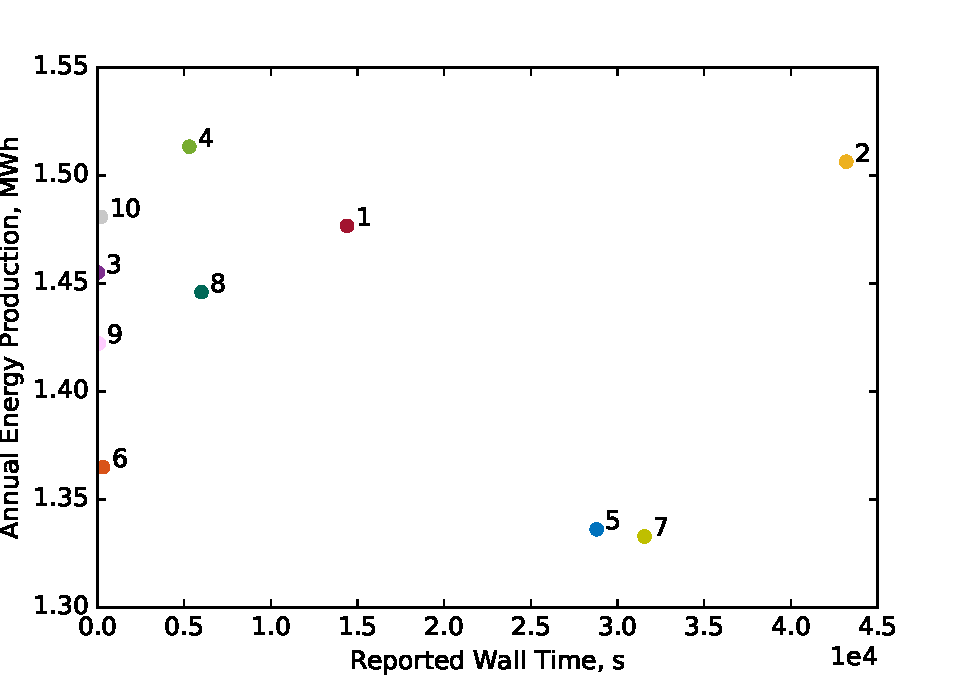
\includegraphics[width=5in]{./figures/AEP_vs_time.pdf}
	    \caption{AEP vs wall time, 64 turbine scenario. Submission numbers placed next to reported values.}
	    \label{fig:AEPvTime}
	\end{figure}
	%\captionsetup[table]{singlelinecheck=on}	% return to normal caption alignment

% 	\newpage
	\import{./sections/}{iea37-wflocs-rslts-cmbnd.tex}

%---- Eduardo's stuff --%
%As this research progresses, a validation of the propeller-on-propeller interactions predicted by VPM will be performed in three phases:

%\begin{enumerate}
%	\item Modeling of the exact experimental setup used in the PIV measurements reported by Zhou \textit{et al.}\cite{Zhou2017} and comparison of the predicted velocity field of this two co-rotating propellers.
%	\item Sweeping of separation distance between the two co-rotating propellers used by Zhou \textit{et al.} and comparison between measured and predicted aerodynamic performance (thrust and torque).
%	\item Once validity is established, we will perform a parametric study of performance on APC 10x7 propellers interacting at varying advance ratios, Reynolds numbers, and separation distance, in counter and co-rotation configurations.
%\end{enumerate}

%With the development and validation of the method presented in this study we aim to show the capabilities of the VPM to model propeller-on-propeller interactions in a first-principles-based approach, with an accuracy and speed well fit for the conceptual design of distributed-propulsion aircraft.